% \begin{figure}[H]
% 	\centering
% 	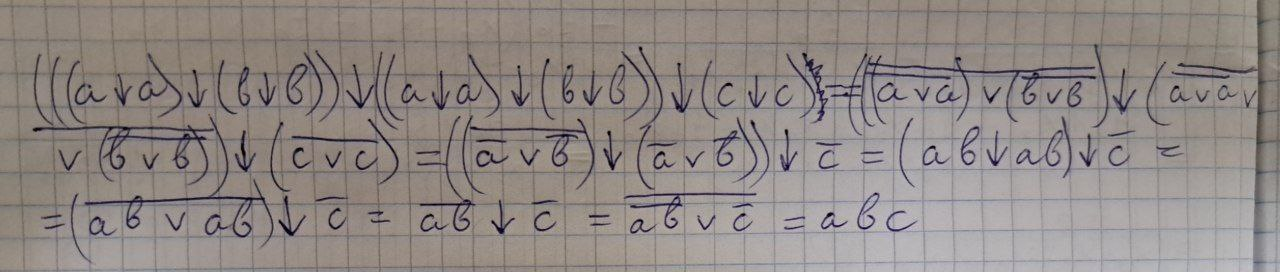
\includegraphics[width=1\textwidth]{../data/formula}
% 	\caption{Вывод схемы БОЭ}
% \end{figure}

\subsubsection{Вывод схемы БОЭ}

Для каждого выхода \( Z_i \) на основе таблицы истинности строим логическое выражение в базисе ИЛИ-НЕ.

### Выражение для \( Z_0 \):
\[
	\begin{gathered}
		Z_0 = \overline{S_1} \cdot \overline{S_0} \cdot Y = \overline{(S_0 \vee S_1) \vee \overline{Y}} = (\overline{\overline{S_0 \vee S_1}}) \vee \overline{Y} \\
		Z_0 = ((S_0 \downarrow S_1) \downarrow (S_0 \downarrow S_1)) \downarrow (Y \downarrow Y)
	\end{gathered}
\]

### Выражение для \( Z_1 \):
\[
	\begin{gathered}
		Z_1 = \overline{S_1} \cdot S_0 \cdot Y = \overline{(S_1 \vee \overline{S_0}) \vee \overline{Y}} = (\overline{S_1 \vee \overline{S_0}}) \vee \overline{Y} \\
		Z_1 = ((S_1 \downarrow (S_0 \downarrow S_0)) \downarrow (S_1 \downarrow (S_0 \downarrow S_0))) \downarrow (Y \downarrow Y)
	\end{gathered}
\]

### Выражение для \( Z_2 \):
\[
	\begin{gathered}
		Z_2 = S_1 \cdot \overline{S_0} \cdot Y = \overline{(\overline{S_1} \vee S_0) \vee \overline{Y}} = (\overline{\overline{S_1} \vee S_0}) \vee \overline{Y} \\
		Z_2 = (((S_1 \downarrow S_1) \downarrow S_0) \downarrow ((S_1 \downarrow S_1) \downarrow S_0)) \downarrow (Y \downarrow Y)
	\end{gathered}
\]

### Выражение для \( Z_3 \):
\[
	\begin{gathered}
		Z_3 = S_1 \cdot S_0 \cdot Y = \overline{(\overline{S_1} \vee \overline{S_0}) \vee \overline{Y}} = (\overline{\overline{S_1} \vee \overline{S_0}}) \vee \overline{Y} \\
		Z_3 = (((S_1 \downarrow S_1) \downarrow (S_0 \downarrow S_0)) \downarrow ((S_1 \downarrow S_1) \downarrow (S_0 \downarrow S_0))) \downarrow (Y \downarrow Y)
	\end{gathered}
\]

Таким образом, конечные формулы для каждого \( Z_i \) выражены в базисе ИЛИ-НЕ, что соответствует структуре демультиплексора 1 в 4 на базе логического элемента NOR.

Реализация этих логических выражений с использованием NOR-вентиля выглядит следующим образом:

1. Для инверсии сигналов \( S_1 \) и \( S_0 \) используются NOR-вентиля с одинаковыми входами:
\[
	\overline{S_0} = NOR(S_0, S_0), \quad \overline{S_1} = NOR(S_1, S_1)
\]

2. Логические операции для каждого выхода можно развернуть через NOR следующим образом:

\[
	Z_0 = NOR(NOR(NOR(S_1, S_0), NOR(S_1, S_0)), NOR(Y, Y))
\]
\[
	Z_1 = NOR(NOR(NOR(S_1, \overline{S_0}), NOR(S_1, \overline{S_0})) , NOR(Y, Y))
\]
\[
	Z_2 = NOR(NOR(NOR(\overline{S_1}, S_0), NOR(\overline{S_1}, S_0)) , NOR(Y, Y))
\]
\[
	Z_3 = NOR(NOR(NOR(\overline{S_1}, \overline{S_0}), NOR(\overline{S_1}, \overline{S_0})) , NOR(Y, Y))
\]

Таким образом, каждый выход \( Z_i \) активен при соответствующей комбинации управляющих сигналов \( S_1, S_0 \), что реализует функцию демультиплексора на базе NOR-вентиля.

\subsubsection{Схема БОЭ}

\begin{figure}[H]
	\centering
	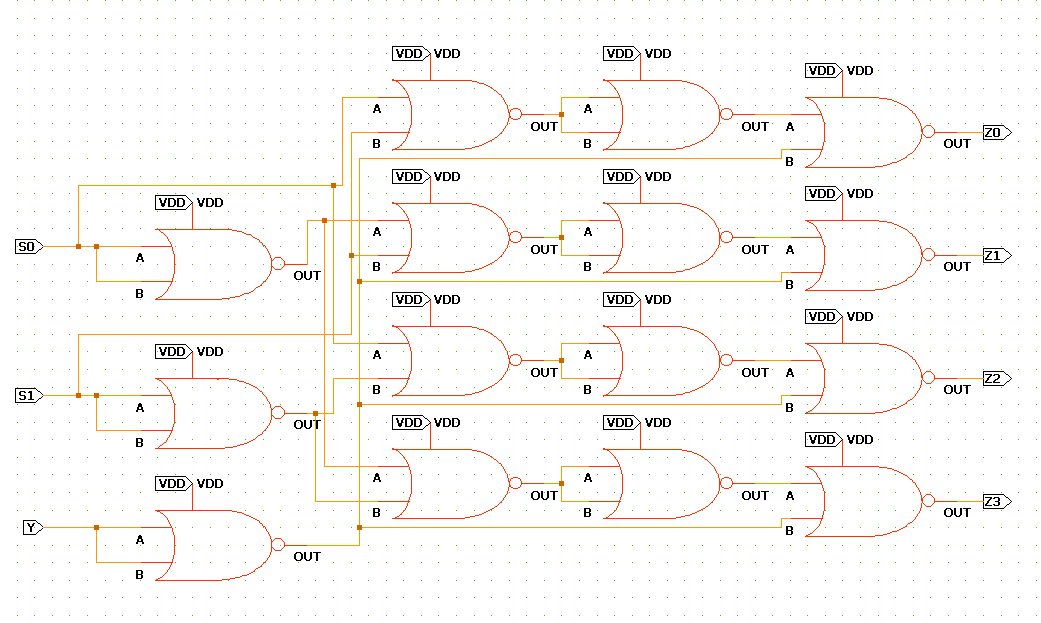
\includegraphics[width=1\textwidth]{../data/demultiplexer_1_to_4}
	\caption{Демультиплексор «1 в 4»}
\end{figure}
